% chapters/ch1_introduction.tex — 第 1 章 绪论
%
% 2026-11-10 成文（目标 3,000 字；1.1 复用归档草稿并补现役证据，1.2/1.3 重写）。
% 写作纪律：WRITING_RULES.md（每千字冒号≤3 / 破折号≤2 / 括号≤4；禁分点；句长变化；
% 章首不写「本章将介绍」，章末不写复述式小结）；数字须可追溯到 results/evidence 工件。
% 结构：1.1 研究背景与意义 / 1.2 国内外研究现状 / 1.3 本文研究内容 / 1.4 论文组织结构。
% 与会议论文的关系：不直接翻译粘贴（OUTLINE.md §六）；贡献强度按大论文展开。

\chapter{绪论}
\label{ch:intro}

\section{研究背景与意义}

自主系统把增强现实、移动机器人与自动驾驶并列为视觉同时定位与建图的主要推进力
\cite{wang2024dynamicsurvey}。三者对定位与建图的要求高度重叠，也都把环境中有人走动当作常态。
这些要求叠在一起，恰好划出了本文要补的那道缺口。

增强现实的定义性要求是把虚拟内容与真实世界在时空上对齐\cite{azuma1997ar}。对齐失准，
虚拟物体就浮在环境表面之外，沉浸感与任务价值同时消失。对齐的载荷压在设备自定位上，
而自定位的质量上限由地图决定。行人从镜头前走过，家具被挪动，门扇开合，静态地图与
真实场景的偏差会直接转成注册误差。更麻烦的是虚实遮挡，虚拟物体要被真实行人正确遮挡，
地图不但得稠密可渲染，还得知道哪些几何此刻可信。这已经不是单纯的定位问题。

移动机器人的处境类似。仓库、商场、家庭这些工作场景都是人机共享的高动态环境，
机器人需要稠密地图做避障与操作规划。动态环境综述把运动物体引入的几何不一致列为
视觉 SLAM 的主要误差源，也把处理它看作从实验室走向部署的分水岭\cite{saputra2018survey}。
被行人污染的特征关联轻则放大定位噪声，重则把行人几何固化进地图，于是一条规划路径
可能直接穿过人的身体。导航安全要求地图持续反映世界现在的样子。

数字孪生与内容创建提出第三组约束。从一段视频重建可编辑的场景模型，表示必须显式且可操作。
补一个静态点云无法支持重光照与增删，隐式神经场的编辑代价又偏高。显式基元表示的可编辑性
在这里成为硬指标，插入、更新与删除都以基元为单位进行。

三类应用的共同要求可以压成一句话，实时、稠密、可渲染、可编辑，并且随动态内容在线更新。
传统稀疏特征点 SLAM 的服务范围覆盖不到这些要求，其地图是稀疏路标，既不支撑渲染，
也没有基元级的编辑面。神经辐射场与三维高斯泼溅支撑的稠密视觉 SLAM 正是在缺口上起来的。
其中随动态内容在线更新这一条最新，也是本文的主战场。

把镜头拉近到具体装置，问题的量级会变得非常直观。本文基座在动态基准的人群序列上
漂移 86.5 与 147.5\,cm（第三章表 3.1 的 MonoGS 未修改基线），静态场景只有约 1.5\,cm。
同一条管线换一个场景，误差跳了两个数量级。这说明动态内容处理
不是锦上添花的模块，而是从实验室到部署的第一道门槛，它的质量同时决定定位精度与地图可用性。

选三维高斯泼溅作表示，原因是它同时给出两个操作面。显式高斯基元支持实时光栅化渲染，
渲染损失可以直接作用在跟踪与建图上；逐基元结构又支持插入、剪枝与生命周期管理，
动态内容的在线增删因此有了物理落点。这两点是隐式表示不具备的。单目设置最普适，
单摄像头即可工作，也最难，深度尺度不定且与动态判定耦合。本文的实验主线放在 RGB-D 基座上，
先把尺度变量隔离出去，单目扩展留作展望。

\section{国内外研究现状}

动态三维高斯泼溅 SLAM 的文献可以按两条路线读。一条把动态当干扰移除或降权，
另一条显式建模动态本身。两条路线各自解决了不同问题，也都留下了相同的盲区。

移除路线的语义先验档以 WildGS-SLAM 为代表，它用 DINOv2 级预训练特征构造逐像素不确定性，
再以马氏距离把不确定观测降权进跟踪损失，在 Bonn 上达到 2.31\,cm。这类方法精度好，
代价是依赖外部大模型，且动态类别先验换一个数据集就要重验。免语义档换用光流与几何一致性
判别，Dy3DGS-SLAM 与 GGD-SLAM 是其中代表，它们摆脱了类别先验，精度普遍落后一档。
免类别先验且精度仍有竞争力的动态判别，目前仍不完整，这是本文研究内容一的入口。

建模路线把动态内容显式写成可演化的基元或形变场。单目设置下实时性与深度尺度两个问题
都还没有一起解决。把 4D 表示搬进在线 SLAM 的尝试不少，能同时守住帧率与 ATE 的不多。
这条路线给本文的启示在表示层，动态基元需要自己的时间参数化，而不是靠逐帧重建去追。

地图管理是第三条容易被忽略的线索。高斯地图在运行结束后如何压缩、修复与继续维护，
决定了它能否从系统输出的副产品变成可独立分析的对象。已有工作开始触及生命周期，
MoPe 与 DL-SLAM 都让基元带上了可观测性状态，但提交之后的状态转换仍不完整。
基元在物体移走、遮挡消失或背景重现时如何退出、恢复与补全，现有机制给不出闭环答案。
这构成研究内容三的问题域。

跟踪后端的分野更清楚。优化式方法以逐帧光度优化为主流，MonoGS 一系把它做成了标准范式，
学习式方法以 DROID 类稠密 BA 为主流，Bonn 上 2--8\,cm 这一档几乎都在后者。
优化式方法的短板是长期漂移没有内解，窗口内的约束修不了窗口外的累积误差。
把窗口光度约束嵌进跟踪循环，让修正即时回灌，是研究内容二的出发点。

把两条路线、地图管理与跟踪后端放在一起看，空缺的位置就出来了。动态判定缺一个
免类别先验且精度可用的做法，漂移缺一个循环内解，地图缺一套提交后的状态管理。
本文三个研究内容分别对准这三处。

值得单独说清的是致密化这一环。三维高斯的自适应密度控制决定地图在哪里长大，
原始判据只是屏幕空间位置梯度的均值。静态重建侧已经证明这个统计口径的每个环节都不中性。
Pixel-GS 按覆盖像素数加权，AbsGS 改用同向梯度分量，StopThePop 从排序入手，
CountingContributions 把统计限制在实际贡献渲染的视角。这些修正合起来说明，
致密化统计会系统性地决定高斯长在哪里。本文在大论文第五章对这条轴做了实证刻画，
并把 E 轴调度作为一次完整的机制验证。该验证在预注册判据下于第二阶段止损，
结论降级为配置层结论。这条负结果不进入贡献栏，只作边界与讨论素材。

\section{本文研究内容}

本文把动态高斯 SLAM 的鲁棒性拆成三个层次。观测层回答哪些像素可信，
估计层回答位姿链如何保持一致，表示层回答地图基元如何随场景演化。三个研究内容各对准一层。

第一项工作落在观测层。它做免类别先验的可靠性引导动态跟踪，系统名为 RoGS-SLAM。
它用光流一致性构造逐像素静态置信，以有下界降权替代硬移除，避免把动态目标整块抹掉后
留下空洞。四个组件构成完整系统，均匀关键帧覆盖、Huber IRLS 鲁棒跟踪、光流一致性可靠性信号
与 lineage 生命周期。一百二十次预注册因子消融加三十六次核消融给出了组件必要性的分层结论，
完整配置在 crowd 场景达到 2.2--2.3\,cm，显存约 4.0\,GB。这部分对应大论文第三章，
会议版已录用。

第二项工作落在估计层，做跟踪循环内的在线滑窗光度联合优化，简称 SWBA。它先给出后处理路线
失败的系统证据，按边类型与跨度做四象限分解，各三条种子，结论是漂移事后不可修复。
证据立住之后，把滑窗光度约束嵌进跟踪循环并即时回灌，再叠一层轻量回环与逐帧部署门控。
person\_tracking 上从 13.62\,cm 降到 7.83\,cm，降幅约四成，方差同步收敛。
距五厘米红线仍差 2.83\,cm，这一缺口如实报告。这部分对应第四章。

第三项工作落在表示层，做动态场景高斯地图的时间感知致密化。这一内容的身份是实证表征，
不是机制贡献。它用五条机制链的否证与剂量前沿刻画回答一个问题，在具备逐事件窗口
自调节的管线里，外置的致密化干预还能不能带来净收益。答案是低 churn 序列上没有，
高 churn 序列仍是开放区。地图规模对剂量的响应在三类序列上普适，渲染质量在低剂量端
随地图坍缩同步下降。这部分对应第五章，结论只以边界与讨论身份存在。

三个层次之间有明确的承接关系。观测层残留的失效，例如 person\_tracking 家族上仍存在的
跟踪误差，恰好是估计层的入口问题。估计层给出的稳定位姿，又是表示层判别基元状态的可信基准。
层层递进之后，第五章的致密化刻画才有干净的测量条件。

\begin{figure}[t]
  \centering
  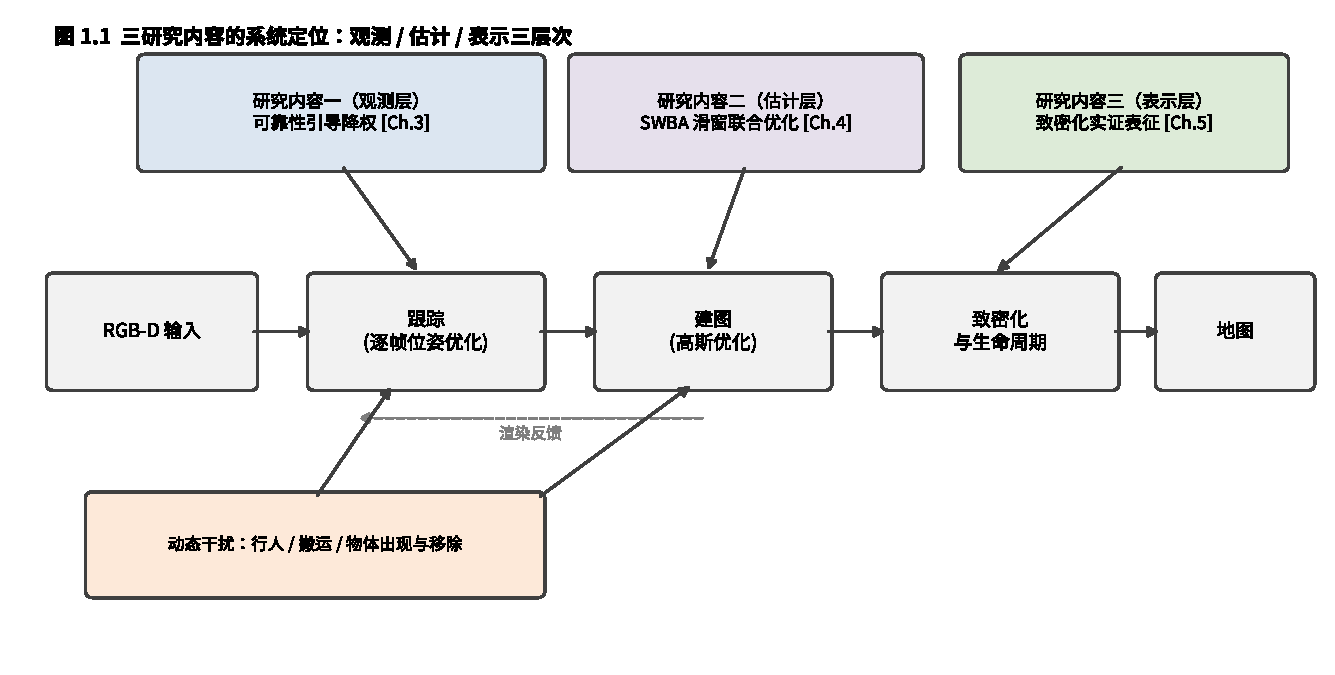
\includegraphics[width=0.95\textwidth]{figures/fig1_architecture.pdf}
  \caption{三研究内容的系统定位。观测层处理哪些像素可信，估计层处理位姿链的一致性，
    表示层处理地图基元的演化。三层沿 RGB-D 输入到地图的流水线依次承接，
    动态干扰自下而上进入跟踪与建图。}
  \label{fig:ch1-architecture}
\end{figure}

\section{论文组织结构}

全文共六章。第一章交代背景、现状、三个研究内容与组织结构。第二章给出相关工作，
沿致密化判据、动态高斯 SLAM、运行后地图的压缩与维护三条线展开。第三章对应研究内容一，
第四章对应研究内容二，第五章对应研究内容三。第六章总结全文并讨论后续方向。
各章数字的来源批次与序列集合在对应表脚注中逐项注明，口径不混引。
